\documentclass[10pt]{article}
\usepackage[utf8]{inputenc}
\usepackage[activeacute,spanish]{babel}
\usepackage[left=1.5cm,top=1.5cm,right=1.5cm, bottom=1.5cm,letterpaper, includeheadfoot]{geometry}

\usepackage{amssymb, amsmath, amsthm}
\usepackage{graphicx}
\usepackage{hyperref}
\usepackage{lmodern,url}
\usepackage{paralist} %util para listas compactas
\usepackage{xcolor}
\usepackage{bbm}
\usepackage{mathrsfs}
\usepackage{bbm}

%========PAQUETES AGREGADOS===========
%Pseudocodigo
\usepackage{pseudocode}
\usepackage[portuguese, boxruled]{algorithm2e}
\usepackage{wrapfig}
\usepackage{multicol}
\usepackage{graphicx}
\usepackage{caption}
\usepackage{subcaption}
%\captionsetup[table]{labelformat=empty}
\captionsetup[subfigure]{labelformat=empty}
\usepackage{cancel}
\usepackage{tikz}
\def\checkmark{\tikz\fill[scale=0.4](0,.35) -- (.25,0) -- (1,.7) -- (.25,.15) -- cycle;} 
%====================================

\usepackage{fancyhdr}
\pagestyle{fancy}
\fancypagestyle{plain}{%
\fancyhf{}
\lhead{\footnotesize\itshape\bfseries\rightmark}
\rhead{\footnotesize\itshape\bfseries\leftmark}
}


% macros
\newcommand{\Q}{\mathbb Q}
\newcommand{\R}{\mathbb R}
\newcommand{\N}{\mathbb N}
\newcommand{\Z}{\mathbb Z}
\newcommand{\C}{\mathbb C}
\newcommand{\BigO}{\mathcal{O}}
%Teoremas, Lemas, etc.
\theoremstyle{plain}
\newtheorem{teo}{Teorema}
\newtheorem{lem}{Lema}
\newtheorem{prop}{Proposición}
\newtheorem{cor}{Corolario}
\newtheorem{obs}{Observación}
\newtheorem{ej}{Ejemplo}
\renewcommand{\qedsymbol}{\rule{0.7em}{0.7em}}
\renewenvironment{proof}{{\bfseries \noindent Demostración}}{ \qed \\}


\theoremstyle{definition}
\newtheorem{defi}{Definición}
% fin macros


\newcommand{\catnum}{20} %numero de catedra
\newcommand{\fecha}{17 de Noviembre 2016 }

%%%%%%%%%%%%%%%%%%

%Macros para este documento
\newcommand{\cin}{\operatorname{cint}}



\begin{document}
%Encabezado
\fancyhead[L]{Facultad de Ciencias Físicas y Matemáticas}
\fancyhead[R]{Universidad de Chile}
\vspace*{-1.2 cm}
\begin{minipage}{0.6\textwidth}
\begin{flushleft}
\hspace*{-0.5cm}\textbf{MA3402-1 Estadística. Primavera 2016}\\
\hspace*{-0.5cm}\textbf{Profesor:} Raul Gouet\\
\hspace*{-0.5cm}\textbf{Escriba:} Manuel Cáceres\\
\hspace*{-0.5cm}\textbf{Fecha:} \fecha
\end{flushleft}
\end{minipage}
\begin{minipage}{0.36\textwidth}
\begin{flushright}

\includegraphics[scale=0.3]{imagenes/fcfm_dcc}
\end{flushright}
\end{minipage}
\bigskip
%Fin encabezado

\begin{center}
\LARGE\textbf{Clase \catnum}
\end{center}
\section{Modelo Lineal (simple)}
$\{(x_{i},y_{i}), i = 1\ldots n\}$ en $\mathbb{R}^2$\\
Resolvimos
\begin{align*}
\min_{\alpha, \beta} \sum (y_{i}-\alpha -\beta x_{i})^2
\end{align*}
Problema de ajuste de mínimos cuadrados.
\begin{center}
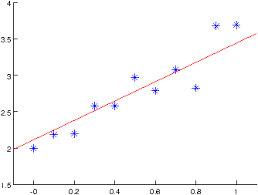
\includegraphics[scale=1]{imagenes/minimosCuadradosLineal.png}
\end{center}
Solución:
\begin{align*}
 \hat{\alpha} &= \bar{y} - \hat{\beta}\bar{x}\\
 \hat{\beta} &= \frac{\frac{1}{n}\sum x_{i}y_{i}- \bar{x}\bar{y}}{\frac{1}{n}\sum x_{i}^2 - \bar{x}^2}\\
 &= \frac{\sigma_{xy}}{\sigma_{x}^2}\\
 &= \frac{\text{covarianza empírica}}{\text{varianza empírica}}
\end{align*}
\section{Hipótesis Probabilística}
Suponemos que los $y_{i}$ son realizaciones de una variable aleatoria $Y_{i}, i = 1\ldots n$, de forma que $\mathbb{E}(Y_{i}) = \alpha + \beta x_{i}$.\\

Entonces, se define la variable aleatoria $\epsilon_{i}$, llamada error, como
\begin{align*}
\epsilon_{i} &= Y_{i} - \mathbb{E}(Y_{i})\\
&= Y_{i} - \alpha - \beta x_{i}
\end{align*}
Claramente $\mathbb{E}(\epsilon_{i}) = 0$.\\

Escribimos $Y_{i} = \alpha + \beta x_{i} + \epsilon_{i}$ que es el modelo lineal simple en estadística.\\

El cálculo de $\alpha$ y $\beta$ será un problema de estimación.\\
Las variables aleatorias $\epsilon_{i}$ no tienen ninguna propiedad(por ahora) excepto $\mathbb{E}(\epsilon_{i}) = 0$.\\
Con esto somos capaces de mostrar que:
\begin{align*}
\hat{\alpha}(Y) &= \bar{Y} - \hat{\beta}(Y)\bar{X}\\
\hat{\beta}(Y) &= \frac{\sigma_{XY}}{\sigma_{X}^2}
\end{align*}
que son insesgados para $\alpha$ y $\beta$ respectivamente.\\

Para continuar buscando propiedades de $\hat{\alpha}$, $\hat{\beta}$ agregamos más hipótesis, que son razonables y luego de los cálculos se pueden confirmar en cierta medida.\\

Supongamos que los $\epsilon_{i}$ tienen varianzas finitas $\mathbb{V}(\epsilon_{i}) = \sigma_{i}^2$ y además son no correlacioneados, es decir, $Cov(\epsilon_{i},\epsilon_{j}) = 0$.\\

Con esto se puede avanzar bastante en los cálculos de $\mathbb{V}(\hat{\alpha})$ y $\mathbb{V}(\hat{\beta})$. Así como $Cov(\hat{\alpha},\hat{\beta})$, sin embargo los $\sigma_{i}$ surgen como nuevos parámetros del modelo, que se agregan a $\alpha$, y $\beta$, teniendo solo $n$ datos.\\

Se suele agregar a lo anterior la hipótesis $\sigma_{i} = \sigma_{j} = \sigma$ , llamada \underline{homocedasticidad}.\\

Resumiendo, pedimos :
\begin{itemize}
\item $\epsilon_{i}$ sean centrados.
\item $\epsilon_{i}$ no correlacionados.
\item $\epsilon_{i}$ con varianzas iguales y finitas.
\end{itemize}
Aún así, no sabemos nada (más) de la esperanza conjunta de $\epsilon_{i}$, que podrían ser dependientes.\\

Ahora si el problema de estimar $\alpha,\beta,\sigma^2$ con $n$ datos es razonable.\\

\section{¿Cómo seguimos?}
\begin{center}
imagenes/puntosNormal
\end{center}
Consideremos un modelo cuadrático.\\

Digamos que:
\begin{align*}
Y_{i} &= \alpha + \beta x_{i} + \gamma x_{i}^2 + \epsilon_{i}
\end{align*}

Planteamos 
\begin{align*}
\min_{\alpha,\beta,\gamma} \sum (y_{i}-\alpha -\beta x_{i} -\gamma x_{i}^2)^2
\end{align*}

Resolvemos buscando puntos estacionarios
\begin{align*}
\frac{\partial}{\partial \alpha} = 0 \Leftrightarrow & \sum (y_{i}-\alpha-\beta x_{i} -\gamma x_{i}^2)^2 = 0\\
\Leftrightarrow & \bar{y} - \alpha - \beta \bar{x^2} - \gamma = 0\\
\frac{\partial}{\partial \beta} = 0 \Leftrightarrow & \frac{1}{n}\sum x_{i}y_{i} - \alpha \bar{x} - \beta \frac{1}{n} \sum x_{i}^2 - \gamma \frac{1}{n} \sum x_{i}^3 = 0\\
\frac{\partial}{\partial \gamma} = 0 \Leftrightarrow &  \sum x_{i}^2y_{i} - \alpha\sum x_{i}^2 - \beta \sum x_{i}^3 - \gamma \sum x_{i}^4 = 0
 \end{align*}
 
 Esperamos que este sistema lineal tenga solución (única?).\\
 
 Vamos resolviendo siempre un sistema lineal.\\
 
 Por ejemplo, en una situación general podría ser conveniente reemplazar las funciones $1,x,x^2$ por  $e_{0}(x),e_{1}(x), e_{2}(x)$ y plantear:
 \begin{align*}
 Y_{i} &= \alpha e_{0}(x_{i}) + \beta e_{1}(x_{i}) + \gamma e_{2}(x) + \epsilon_{i}
 \end{align*}
 Y resolvemos 
 \begin{align*}
 \min_{\alpha, \beta, \gamma} \sum (\alpha e_{0}(x_{i}) + \beta e_{1}(x_{i}) + \gamma e_{2}(x) + \epsilon_{i} - y_{i})^2
 \end{align*}
 Buscamos los puntos estacionarios y llegamos al sistema:
 \begin{align*}
 \sum y_{i}e_{0}(x_{i}) - \alpha\sum e_{0}(x_{i}^2) -\beta\sum e_{1}(x_{i})e_{0}(x_{i}) - \gamma\sum e_{2}(x_{i})e_{1}(x_{1})e_{0}(x_{i})\\
 \sum y_{i}e_{1}(x_{i}) - \alpha \sum e_{0}(x_{i})e_{1}(x_{i}) - \beta\sum e_{i}(x_{i})^2 - \gamma \sum e_{1}(x_{i})e_{2}(x_{i}) = 0\\
 \ldots
 \end{align*}
 
 En general, para ajustar modelos de dependencia más complejos, consideramos funciones $e_{1}(x), e_{2}(x),\ldots, e_{n}(x)$ y  escribimos
 \begin{align*}
 Y_{i} &= \beta_{1}e_{1}(x_{i}) + \beta_{2}e_{2}(x_{i}) + \ldots + \beta_{n} e_{n}(x_{i}) + \epsilon_{i}
 \end{align*}
 Luego lo que hacemos es
 \begin{align*}
 \min_{\beta_{1},\beta_{2},\ldots, \beta_{n}} \sum_{i=1}^n \left(y_{i} - \sum_{j=1}^k \beta_{j} e_{j}(x_{i}\right)^2\\
\frac{\partial}{\partial \beta_{i}} = 0 \Leftrightarrow \sum_{i=1}^n \left(y_{i}- \sum_{l}\beta_{l}e_{l}(x_{i})\right)e_{j}(x_{i}) = 0
 \end{align*}
 
 Hay efectivamente situaciones de no linealidad (ya veremos)\\
 
 ¿Qué ocurre si tenemos más de una variable explicativa x? Por ejemplo, $y$ depende del fertilizante $x$  y la humedad $u$. Digamos entonces:
 \begin{align*}
 Y_{i} = \alpha + \beta x_{i} + \gamma u_{i} + \epsilon
 \end{align*}
 \begin{center}
 imagenes/ gráfico n R3 con plano óptimo
 \end{center}
 Resolvemos 
 \begin{align*}
 \min_{\alpha,\beta,\gamma} \sum (y_{i}- \alpha - \beta x_{i} - \gamma u_{i})^2\\
\frac{\partial}{\partial \alpha} = 0\\
\frac{\partial}{\partial \beta} = 0\\
\frac{\partial}{\partial \gamma} = 0\\
 \end{align*}
 Que es un sistema lineal.
 \section{Modelo lineal general}
 Aquí consideramos $k$ variables de tipo explicativa $x$, con las cuales intentamos reconstruir linealmente a $y$.\\
 
 Tenemos el modelo
 \begin{align*}
 Y_{i} = \sum_{j=1}^k \beta_{j} \underbrace{x_{ij}}_{\text{iésimo valor de la variable j}} + \epsilon_{i}
 \end{align*}
 Resolvemos
 \begin{align*}
 \min_{\beta_{1},\beta_{2},\ldots, \beta_{n}} \sum_{i=1}^n (y_{i}- \sum_{j=1}^k \beta_{j}x_{ij})^2
 \end{align*}
 La nube $(x_{i1},x_{i2},\ldots,x_{ik}, y_{i})_{i=1\ldots n}$ está en $\mathbb{R}^{k+1}$.\\
 La idea es ajustar hiperplano a la nube.
 \section{Notación Matricial}
 Se definen las siguientes matrices (y vectores):
 \begin{align*}
    Y &= \begin{bmatrix}
           Y_{1} \\
           Y_{2} \\
           \vdots \\
           Y_{n}
         \end{bmatrix}
  \end{align*}
  Vector $n\times 1$ aleatorio (observaciones)
  \begin{align*}
    \epsilon &= \begin{bmatrix}
           \epsilon_{1} \\
           \epsilon_{2} \\
           \vdots \\
           \epsilon_{n}
         \end{bmatrix}
  \end{align*}
  Vector $n\times 1$ aleatorio (errores)
    \begin{align*}
    \beta &= \begin{bmatrix}
           \beta_{1} \\
           \beta_{2} \\
           \vdots \\
           \beta_{k}
         \end{bmatrix}
  \end{align*}
  Vector $k\times 1$ de los parámetros del modelo (fuera de $\sigma$).\\
  
  Los valores $x_{ij}$ de las variables explicativas se agrupan en la matriz de $n\times k$
  \begin{align*}
  X = (x_{ij})_{i=1\ldots n, j=1\ldots k}
  \end{align*}
  En términos matriciales, el modelo lineal general se escribe como
  \begin{align*}
  Y = X \beta + \epsilon
  \end{align*}
  Recordemos que para vectores o matrices aleatorias, digamos $Z = (z_{ij})$, se tiene:
  \begin{align*}
  \mathbb{E}(Z) = (\mathbb{E}(Z_{ij}))
  \end{align*}
  Propiedades, si $A$ y $B$ son matrices no aleatorias, entonces:
  \begin{align*}
  \mathbb{E}(AZ) &= A \mathbb{E}(Z)\\
  \mathbb{E}(ZB) &= \mathbb{E}(Z) B
  \end{align*}
  Notación en $\mathbb{R}^n$, si
 \begin{align*}
    y &= \begin{bmatrix}
           y_{1} \\
           y_{2} \\
           \vdots \\
           y_{n}
         \end{bmatrix}
  \end{align*}
, $y' = (y_{1},y_{2},\ldots, y_{n})$\\
\begin{align*}
||y||^2 = \sum_{i=1}^n y_{i}^2 = y'y = <y,y>
\end{align*}  
El problema a resolver es
\begin{align*}
& \min_{\beta_{1},\ldots, \beta_{k}} \sum_{i=1}^n (\underbrace{Y_{i}-\sum \beta_{j} x_{ij}}_{\epsilon^2})^2\\
& \Leftrightarrow \min_{\beta} \sum \epsilon_{i}^2\\
& \Leftrightarrow \min_{\beta} ||\epsilon||^2\\
& \Leftrightarrow \min_{\beta} ||Y-X\beta||^2\\
& \Leftrightarrow \min_{\beta} (Y-X\beta)'(Y-X\beta)
\end{align*}

El problema $\min_{\beta} ||Y-X\beta||^2$ es un problema de proyección!!.\\

Porque cuando $\beta$ recorre $\mathbb{R}^k$, $X\beta$ recorre el subespacio engendrado por las columnas de $X$.\\
Sea $<X>$ el subespacio vectorial de $\mathbb{R}^n$ engendrado por las columnas de $X$.\\
Entonces $||Y-X\beta||^2$ se minimiza cuando $X\hat{\beta}$ es la proyección de $Y$ en $<X>$.
\end{document}
